\documentclass[conference]{IEEEtran}
\IEEEoverridecommandlockouts

\usepackage{cite}
\usepackage{amsmath,amssymb,amsfonts}
\usepackage{graphicx}
\usepackage{textcomp}
\usepackage{xcolor}
\usepackage{booktabs}
\usepackage{multirow}
\usepackage{hyperref}
\usepackage{url}
\usepackage{float}
\usepackage{tikz}
\usetikzlibrary{positioning, arrows.meta}

\begin{document}

\title{FurnishRAG: A Retrieval-Augmented Generation System for IKEA Buying Guides with Chunking Strategy Comparison}

\author{
\IEEEauthorblockN{Tatiana Teixeira}
\IEEEauthorblockA{\textit{MEDados -- MINTRI} \\
\textit{ISEP -- Polytechnic of Porto}\\
Porto, Portugal \\
1221260@isep.ipp.pt}
\and
\IEEEauthorblockN{Rodrigo Pacheco}
\IEEEauthorblockA{\textit{MEDados -- MINTRI} \\
\textit{ISEP -- Polytechnic of Porto}\\
Porto, Portugal \\
1221900@isep.ipp.pt}
}

\maketitle

\begin{abstract}
We present FurnishRAG, a Retrieval-Augmented Generation system designed to answer questions about IKEA furniture products using a corpus of 20 buying guides. The system implements hybrid retrieval combining dense vector search with BM25 scoring through Reciprocal Rank Fusion, and compares three chunking strategies: fixed-size (512 tokens), semantic (embedding-based breakpoints), and hierarchical parent-child (128/1024 tokens). We evaluate all strategies across 30 gold-standard queries spanning factual, comparative, and thematic categories, measuring retrieval quality (MRR, nDCG@5, Recall@5, Precision@5), answer quality (correctness, faithfulness, completeness), and intrinsic chunk metrics (ICC, ICD). Results show that fixed-size chunking achieves the best overall retrieval (MRR\,=\,0.811) and answer correctness (0.642), while semantic chunking leads in faithfulness (0.802). The hierarchical approach underperforms on this corpus (MRR\,=\,0.656), which we attribute to the flat document structure of buying guides. We also integrate five text mining features---keyword extraction, topic modelling, clustering, taxonomy classification, and summarization---to provide exploratory analysis beyond basic question answering.
\end{abstract}

\begin{IEEEkeywords}
retrieval-augmented generation, chunking strategies, information retrieval, text mining, hybrid retrieval, evaluation
\end{IEEEkeywords}

% ============================================================
\section{Introduction and Problem Definition}

Customers shopping for IKEA furniture often need to consult multiple buying guides to find product dimensions, compare storage systems, or plan room layouts. These guides---typically 4--12 page PDFs---contain detailed specifications, compatibility notes, and planning advice that are difficult to cross-reference manually. A standalone large language model (LLM) cannot reliably answer questions about specific IKEA products because it lacks access to the actual guide content and tends to fabricate measurements and product names when asked about details outside its training data. Retrieval-Augmented Generation (RAG)~\cite{b1} addresses this by grounding LLM responses in retrieved document passages.

We designed FurnishRAG to address this problem. The system retrieves relevant passages from a corpus of 20 IKEA buying guides and uses them as grounding context for an LLM, ensuring that answers contain verifiable product information with source citations. Our target users are customers, interior design enthusiasts, and retail staff who need quick, accurate answers about product specifications and compatibility across IKEA product lines.

RAG is appropriate for this task because the information changes frequently (IKEA updates its catalog regularly), the answers require precise numerical specifications (dimensions, load capacities, prices vary by region), and users benefit from seeing which buying guide a claim comes from. A fine-tuned model would quickly become outdated and could not provide source attribution.

Beyond building a working RAG prototype, our engineering goal is to compare three chunking strategies---fixed-size, semantic, and hierarchical---and evaluate how each affects retrieval and answer quality across different query types. This comparison forms the core contribution of this work.

% ============================================================
\section{System Overview}

The system has four main components: (1)~corpus ingestion and preprocessing, (2)~chunking and indexing with three parallel strategies, (3)~hybrid retrieval and LLM generation with anti-hallucination verification, and (4)~text mining features for corpus exploration. Fig.~\ref{fig:pipeline} shows the full pipeline architecture, and Fig.~\ref{fig:overview} compares the three strategies across five key dimensions.

\begin{figure}[htbp]
\centering
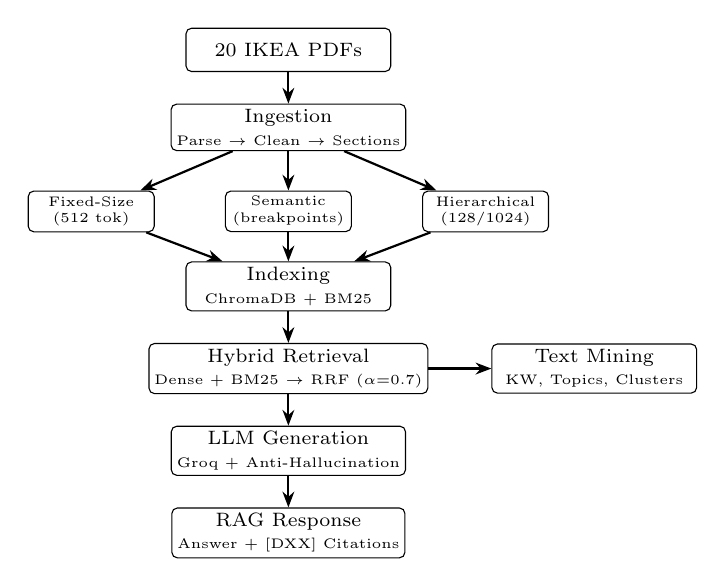
\begin{tikzpicture}[
  node distance=0.4cm,
  box/.style={rectangle, draw, rounded corners=2pt, minimum width=2.6cm, minimum height=0.55cm, align=center, font=\scriptsize},
  smallbox/.style={rectangle, draw, rounded corners=2pt, minimum width=1.6cm, minimum height=0.45cm, align=center, font=\tiny},
  arrow/.style={-{Stealth[length=2mm]}, thick},
  every node/.style={inner sep=2pt}
]
\node[box] (corpus) {20 IKEA PDFs};
\node[box, below=of corpus] (ingest) {Ingestion\\\tiny{Parse $\to$ Clean $\to$ Sections}};
\node[smallbox, below left=0.5cm and 0.2cm of ingest] (fixed) {Fixed-Size\\(512 tok)};
\node[smallbox, below=0.5cm of ingest] (semantic) {Semantic\\(breakpoints)};
\node[smallbox, below right=0.5cm and 0.2cm of ingest] (hier) {Hierarchical\\(128/1024)};
\node[box, below=1.4cm of ingest] (index) {Indexing\\\tiny{ChromaDB + BM25}};
\node[box, below=of index] (retrieve) {Hybrid Retrieval\\\tiny{Dense + BM25 $\to$ RRF ($\alpha$=0.7)}};
\node[box, below=of retrieve] (generate) {LLM Generation\\\tiny{Groq + Anti-Hallucination}};
\node[box, below=of generate] (answer) {RAG Response\\\tiny{Answer + {[DXX]} Citations}};
\node[box, right=0.8cm of retrieve] (tm) {Text Mining\\\tiny{KW, Topics, Clusters}};

\draw[arrow] (corpus) -- (ingest);
\draw[arrow] (ingest) -- (fixed);
\draw[arrow] (ingest) -- (semantic);
\draw[arrow] (ingest) -- (hier);
\draw[arrow] (fixed) -- (index);
\draw[arrow] (semantic) -- (index);
\draw[arrow] (hier) -- (index);
\draw[arrow] (index) -- (retrieve);
\draw[arrow] (retrieve) -- (generate);
\draw[arrow] (generate) -- (answer);
\draw[arrow] (retrieve) -- (tm);
\end{tikzpicture}
\caption{FurnishRAG pipeline architecture. Documents are ingested, split by three chunking strategies, indexed in parallel vector and BM25 stores, and retrieved via hybrid fusion. Text mining features operate on retrieved results.}
\label{fig:pipeline}
\end{figure}

\begin{figure}[htbp]
\centerline{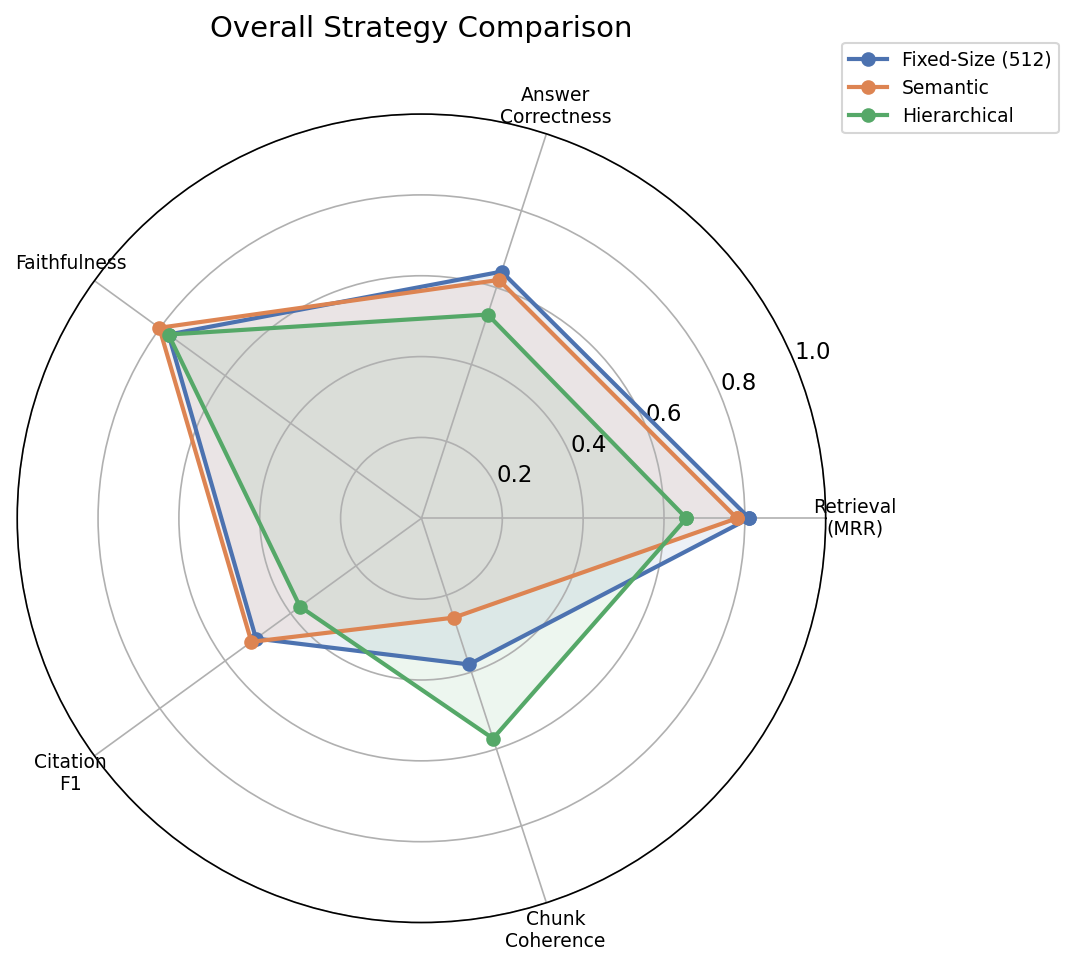
\includegraphics[width=\columnwidth]{figures/overall_strategy_summary.png}}
\caption{Overall strategy comparison across five key dimensions: retrieval quality (MRR), answer correctness, faithfulness, citation F1, and chunk coherence (ICC).}
\label{fig:overview}
\end{figure}

\subsection{Design Decisions}

We chose \textbf{hybrid retrieval} (dense + BM25) because dense retrieval alone can miss exact product names and model numbers, while BM25 alone struggles with paraphrased queries. Reciprocal Rank Fusion (RRF)~\cite{b3} combines both ranking signals without requiring score calibration.

For the LLM, we use \textbf{Groq API} with \texttt{llama-3.1-8b-instant}~\cite{b8} rather than OpenAI models. This decision was driven by cost: the Groq free tier provides sufficient throughput for our 90 evaluation experiments without any API charges. While a larger model would likely improve answer quality, the 8B parameter model is adequate to demonstrate the RAG pipeline and test our chunking hypotheses.

We use \textbf{ChromaDB}~\cite{b9} as the vector store because it supports persistent storage, metadata filtering, and cosine similarity search without requiring an external server. For embeddings, we use the local \textbf{all-MiniLM-L6-v2} model (384 dimensions) from sentence-transformers~\cite{b4}, which runs without API costs and provides reasonable semantic similarity for English text.

The system is implemented in Python without relying on a high-level RAG framework (e.g., LangChain) for the core pipeline. We use LlamaIndex only for its \texttt{SentenceSplitter} tokenizer in the chunking module. This gives us full control over the retrieval and generation logic, which is important for the chunking comparison experiment.

% ============================================================
\section{Corpus and Data Preparation}

\subsection{Dataset Description}

The corpus consists of 20 IKEA buying guides (D01--D20), sourced from IKEA's public websites (IKEA USA, IKEA Canada, IKEA Global). The guides cover five product categories:

\begin{itemize}
    \item \textbf{Storage \& Organization} (4 guides): BILLY, KALLAX, BESTA, EKET
    \item \textbf{Bedroom \& Wardrobe} (5 guides): PAX system, PAX planner, Mattresses, Beds, HEMNES Bedroom
    \item \textbf{Kitchen \& Dining} (3 guides): SEKTION, Kitchen Planning, KUNGSFORS
    \item \textbf{Living \& Outdoor} (4 guides): HEMNES Living Room, KIVIK, EKTORP, BONDHOLMEN
    \item \textbf{Home \& Sustainability} (4 guides): Style Guide, Laundry, Circular Design, Bathroom
\end{itemize}

Each guide is a PDF of 4--12 pages. The total corpus contains approximately 67,000 words after preprocessing.

\subsection{Preprocessing Pipeline}

The ingestion pipeline has three stages:

\textbf{1. PDF Parsing.} We use PyMuPDF (fitz) to extract text page by page. PyMuPDF handles single-column layouts well, which matches the format of most IKEA buying guides (unlike IEEE two-column papers).

\textbf{2. Text Cleaning.} We remove headers, footers, page numbers, URLs, and price references (since prices are region- and time-dependent). Unicode characters are normalized, and excessive whitespace is collapsed. We preserve product names, dimensions, and measurement units.

\textbf{3. Section Detection.} We detect section boundaries using a combination of formatting heuristics (capitalized lines, numbered headings) and IKEA-specific patterns (e.g., ``Good to know'', ``How to choose'', ``Tips''). Detected sections are stored as metadata for each document, which helps with retrieval result interpretation.

\subsection{Chunking Strategies}

Table~\ref{tab:chunking} summarizes the three chunking strategies and the resulting corpus statistics.

\begin{table}[htbp]
\caption{Chunking Strategy Parameters and Corpus Statistics}
\begin{center}
\begin{tabular}{lccc}
\toprule
& \textbf{Fixed-Size} & \textbf{Semantic} & \textbf{Hierarchical} \\
\midrule
Chunk size (tokens) & 512 & variable & child: 128 \\
Overlap (tokens) & 50 & buffer: 1 sent & parent: 1024 \\
Total chunks & 311 & 274 & 1369 \\
Avg tokens/chunk & 237 & 293 & 56 \\
Min tokens & 3 & 3 & 1 \\
Max tokens & 527 & 3493 & 132 \\
\bottomrule
\end{tabular}
\label{tab:chunking}
\end{center}
\end{table}

\textbf{Strategy 1: Fixed-Size} splits text into chunks of 512 tokens with 50-token overlap using LlamaIndex's \texttt{SentenceSplitter}, which respects sentence boundaries. We chose 512 tokens as it is the most commonly used chunk size in RAG literature and provides a reasonable balance between context and specificity. The 50-token overlap prevents information loss at chunk boundaries.

\textbf{Strategy 2: Semantic} splits text at points where consecutive sentence embeddings show a large cosine distance, indicating a topic shift. We use the 95th percentile of inter-sentence distances as the breakpoint threshold. This produces variable-size chunks that are semantically coherent but can be very large (up to 3493 tokens) or very small. We included this strategy to test whether semantic coherence at the chunk level translates to better retrieval performance.

\textbf{Strategy 3: Hierarchical Parent-Child} creates two levels of chunks. Small \textit{child} chunks (128 tokens) are indexed and used for retrieval matching---their small size provides precise term matching. When a child chunk is retrieved, the system returns its \textit{parent} chunk (1024 tokens) to the LLM, providing richer generation context. This decoupled design separates the retrieval unit from the generation unit, addressing the precision-context trade-off: smaller chunks are better for matching, but larger chunks provide more context for answer generation.

\subsection{Intrinsic Chunk Quality Metrics}

We computed four intrinsic metrics to characterize chunk quality before any retrieval evaluation (Table~\ref{tab:intrinsic}).

\begin{table}[htbp]
\caption{Intrinsic Chunk Quality Metrics (sample of 100 chunks)}
\begin{center}
\begin{tabular}{lccc}
\toprule
\textbf{Metric} & \textbf{Fixed} & \textbf{Semantic} & \textbf{Hierarchical} \\
\midrule
ICC (coherence) $\uparrow$ & 0.380 & 0.258 & 0.573 \\
ICD (distinctiveness) $\uparrow$ & 0.376 & 0.423 & 0.446 \\
SC (size compliance) $\downarrow$ & 0.459 & 1.314 & 0.583 \\
BC (boundary clarity) $\uparrow$ & 0.580 & 0.931 & 0.469 \\
\bottomrule
\end{tabular}
\label{tab:intrinsic}
\end{center}
\end{table}

\textbf{Intra-Chunk Coherence (ICC)} measures the average cosine similarity between consecutive sentences within a chunk. Higher values indicate more topically coherent chunks. Hierarchical children (0.573) are the most coherent because they are small enough to cover a single topic, while semantic chunks (0.258) are surprisingly the least coherent---likely because the variable chunk sizes include some very large chunks that span multiple sub-topics.

\textbf{Inter-Chunk Distinctiveness (ICD)} measures 1 minus the cosine similarity between adjacent chunks. Higher values mean chunks are more distinct from each other. Hierarchical (0.446) and semantic (0.423) both outperform fixed-size (0.376), which makes sense since fixed-size splitting is content-agnostic.

\textbf{Size Compliance (SC)} measures the variance in chunk sizes. Lower values indicate more uniform chunks. Semantic chunking has the highest variance (1.314) due to its variable-size nature, while fixed-size has the lowest (0.459), as expected.

\textbf{Boundary Clarity (BC)} measures the semantic discontinuity at chunk boundaries. Semantic chunking achieves the highest BC (0.931), confirming that it does place boundaries at topic shifts. Fixed-size (0.580) and hierarchical (0.469) have lower boundary clarity because their split points are determined by token count rather than content.

% ============================================================
\section{Retrieval Component}

\subsection{Hybrid Retrieval with RRF}

We implement hybrid retrieval combining dense vector search and BM25~\cite{b2} lexical matching through Reciprocal Rank Fusion (RRF)~\cite{b3}. For a given query, both retrievers return their top-$2k$ results (where $k$ is the desired number of final results), and RRF computes a fused score:

\begin{equation}
\text{score}(d) = \alpha \cdot \frac{1}{k_{\text{rrf}} + r_{\text{dense}}} + (1-\alpha) \cdot \frac{1}{k_{\text{rrf}} + r_{\text{bm25}}}
\end{equation}

\noindent where $r_{\text{dense}}$ and $r_{\text{bm25}}$ are the ranks of document $d$ in each retriever's results, $k_{\text{rrf}}=60$ is the RRF constant, and $\alpha=0.7$ gives higher weight to dense retrieval. The top-$k$ documents by fused score are returned.

We set $\alpha=0.7$ to favor dense retrieval because our queries are often paraphrased (e.g., ``storage capacity'' instead of ``maximum load''), where semantic similarity is more useful than exact term matching. However, BM25 remains important for queries containing exact product names (e.g., ``KALLAX'', ``SEKTION'') that the embedding model may not distinguish well from semantically similar but different products.

\subsection{Hierarchical Retrieval}

For the hierarchical strategy, the retriever operates differently. The dense index and BM25 index contain the 1369 \textit{child} chunks (128 tokens each). When a child chunk is matched, the system looks up its \textit{parent} chunk (1024 tokens) and returns the parent text to the LLM instead. This means the LLM receives broader context than what the retriever matched on.

\subsection{Example Retrieved Documents}

For the query ``What are the available frame widths for the PAX wardrobe system?'', the hybrid retriever returns 5 chunks. The top-ranked chunk (from D02, PAX Wardrobe Buying Guide, section ``Pick your style'') contains the exact answer: frame widths of 19\textonehalf{}'', 29\textonehalf{}'', and 39\textonequarter{}''. The retriever correctly identifies D02 as the primary source with an RRF score of 0.0164.

For comparative queries like ``Compare the PAX wardrobe and BESTA storage system in terms of available sizes'', the retriever sometimes fails to retrieve all relevant documents. In the fixed-size strategy, this query retrieved D02 (PAX) but missed D04 (BESTA), leading to an incomplete answer. This is a known limitation of top-$k$ retrieval when a query requires information from multiple distinct documents.

% ============================================================
\section{Generation Component}

\subsection{LLM and Prompt Design}

We use \texttt{llama-3.1-8b-instant} via the Groq API with temperature\,=\,0.1 and max\_tokens\,=\,1024. The prompt consists of a system message and a user message. The system message instructs the model to act as a furniture assistant, base every claim on the retrieved context, cite sources as [DXX] notation, and never fabricate product specifications. The user message provides the retrieved context (numbered sources with document ID and section metadata) followed by the question.

Context is injected by concatenating the retrieved chunks with their source metadata:

\begin{verbatim}
[Source 1: D02, Section: Pick your style]
<chunk text>
[Source 2: D20, Section: Pick your style]
<chunk text>
...
\end{verbatim}

This format allows the LLM to attribute information to specific guides using [DXX] citations, which are then verified programmatically.

\subsection{Anti-Hallucination Guard}

We implement a post-generation verification step that:

\begin{enumerate}
    \item \textbf{Verifies citations}: checks that every [DXX] tag in the answer refers to a document actually present in the retrieved context. Invalid citations are stripped from the answer.
    \item \textbf{Computes confidence}: a heuristic score (0--1) based on retrieval quality (RRF scores), citation presence, source diversity, and answer substance.
    \item \textbf{Triggers refusal}: if confidence falls below 0.3 or all citations are invalid, the system refuses to answer and explains why, rather than presenting an unreliable response.
\end{enumerate}

This guard does not prevent all hallucinations---the LLM can still generate plausible-sounding but incorrect product details within a validly-cited document. However, it catches the most obvious failure modes: answers citing non-retrieved documents and answers with very low retrieval confidence.

% ============================================================
\section{Text Mining Features}

We implement five text mining features that add value beyond basic question answering. These features help users explore the corpus, discover patterns, and understand the relationships between different IKEA product lines.

\subsection{Keyword Extraction}

We use KeyBERT~\cite{b6} with the all-MiniLM-L6-v2 embedding model to extract keywords at three levels: per-section, per-document, and corpus-wide. We enable Maximal Marginal Relevance (MMR) with diversity\,=\,0.7 to reduce redundancy in the extracted keywords. Keyphrase n-gram range is set to (1, 3) to capture both single words and multi-word terms (e.g., ``adjustable shelves'', ``soft closing hinges'').

This feature is useful for quickly understanding what each buying guide covers without reading it entirely. It also reveals which concepts are unique to specific guides versus shared across multiple product lines (e.g., ``wall mounting'' appears in BILLY, BESTA, and EKET guides).

\subsection{Topic Modelling}

We apply BERTopic~\cite{b5} to discover latent topics in the corpus. Since 20 documents are too few for meaningful topic modelling, we run BERTopic on chunks (hundreds of data points) rather than full documents. We use HDBSCAN for clustering with a minimum topic size of 3.

A key output is the \textbf{taxonomy alignment score}: we compare BERTopic's discovered topics against our predefined 5-category IKEA taxonomy (Storage, Bedroom, Kitchen, Living, Home) by measuring how well topic-document assignments match the taxonomy's document-category assignments. This provides an independent validation of whether the taxonomy categories are reflected in the actual text content.

\subsection{Clustering}

We cluster retrieved chunks using KMeans or HDBSCAN over their embedding vectors, with UMAP for dimensionality reduction and 2D visualization. For each set of retrieved results, we compute a \textbf{diversity score} based on three factors: the number of unique source documents represented, the number of distinct sections, and the average pairwise cosine distance between chunk embeddings. A low diversity score for a query's results suggests the retriever is returning redundant information from the same source, which is useful for diagnosing retrieval weaknesses.

\subsection{Taxonomy Classification}

We implement an embedding-based classifier that assigns each chunk to one of the five IKEA product categories. The classifier computes cosine similarity between a chunk's embedding and the embeddings of category descriptions, assigning each chunk to its closest category. This is applied to retrieved results to show users how the answer draws from different product categories---for example, a query about ``bedroom storage'' might retrieve chunks classified as both ``Bedroom \& Wardrobe'' and ``Storage \& Organization''.

\subsection{Summarization}

We implement abstractive summarization using a map-reduce approach. For retrieved chunks, the summarizer first generates a per-chunk summary via the LLM, then combines these into a coherent synthesis focused on the user's query. For full-document summarization, it summarizes each section independently (map step) and then merges the section summaries into a document-level summary (reduce step). The LLM (via Groq) handles all generation steps.

\subsection{Integrated Example}

To illustrate how these features work together, consider the query ``What are the available frame widths for the PAX wardrobe system?'' The retriever returns 5 chunks from 2 documents (D02 and D20). The keyword extractor identifies terms such as \textit{frame widths}, \textit{wardrobe system}, and \textit{sliding doors} from the retrieved chunks. The taxonomy classifier assigns all retrieved chunks to the \textit{Bedroom \& Wardrobe} category, confirming alignment with the query topic. The clustering module computes a diversity score across the 2 unique source documents, indicating that the retriever draws from both the PAX buying guide and the PAX planner guide rather than concentrating on a single source. These features are accessible through the Corpus Explorer page of the Streamlit demo.

% ============================================================
\section{Evaluation and Validation}

\subsection{Evaluation Methodology}

We define 30 gold-standard test queries across three categories, each testing different retrieval and generation capabilities:

\begin{itemize}
    \item \textbf{Factual (F01--F10)}: precise product specifications (e.g., ``What is the maximum load per shelf for the BILLY bookcase?''). Tests retrieval precision and factual extraction.
    \item \textbf{Comparative (C01--C10)}: cross-product comparisons (e.g., ``Compare the PAX wardrobe and BESTA storage system''). Tests retrieval breadth and multi-document synthesis.
    \item \textbf{Thematic (T01--T10)}: synthesis across multiple guides (e.g., ``How does IKEA address sustainability across its product lines?''). Tests deep cross-corpus reasoning.
\end{itemize}

Each query has a manually written gold-standard answer with identified relevant documents. We run all 30 queries against all 3 strategies, producing 90 experiments.

\subsection{Metrics}

We measure performance along two axes:

\textbf{Retrieval quality:}
\begin{itemize}
    \item \textit{MRR} (Mean Reciprocal Rank): position of the first relevant document
    \item \textit{nDCG@5}: ranking quality of the top-5 results
    \item \textit{Recall@5}: fraction of relevant documents found in top-5
    \item \textit{Precision@5}: fraction of top-5 results that are relevant
\end{itemize}

\textbf{Answer quality} (using LLM-as-judge~\cite{b7} with the same Groq model):
\begin{itemize}
    \item \textit{Correctness}: factual agreement with the gold-standard answer
    \item \textit{Faithfulness}: whether claims are supported by the retrieved context
    \item \textit{Completeness}: coverage of key points from the gold standard
    \item \textit{Citation F1}: precision and recall of document citations
\end{itemize}

\subsection{Results}

Table~\ref{tab:results} presents the main results.

\begin{table}[htbp]
\caption{Evaluation Results: 30 queries $\times$ 3 strategies}
\begin{center}
\resizebox{\columnwidth}{!}{%
\begin{tabular}{lcccccccc}
\toprule
\textbf{Strategy} & \textbf{MRR} & \textbf{nDCG} & \textbf{R@5} & \textbf{P@5} & \textbf{Corr.} & \textbf{Faith.} & \textbf{Compl.} & \textbf{Cit.F1} \\
\midrule
Fixed-Size & \textbf{0.811} & \textbf{0.663} & \textbf{0.670} & \textbf{0.463} & \textbf{0.642} & 0.773 & \textbf{0.533} & 0.506 \\
Semantic & 0.781 & 0.649 & 0.652 & 0.436 & 0.620 & \textbf{0.802} & 0.513 & \textbf{0.520} \\
Hierarchical & 0.656 & 0.561 & 0.578 & 0.437 & 0.530 & 0.773 & 0.390 & 0.371 \\
\bottomrule
\end{tabular}}
\label{tab:results}
\end{center}
\end{table}

\textbf{Fixed-size} achieves the best retrieval (MRR\,=\,0.811) and correctness (0.642), along with the highest completeness (0.533). Its consistent chunk sizes produce reliable retrieval behavior. Precision@5 is moderate (0.463) because queries with a single gold document still retrieve 5 chunks.

\textbf{Semantic} chunking is close to fixed-size in retrieval and achieves the highest faithfulness (0.802) and citation F1 (0.520). The semantically coherent chunks may help the LLM stay grounded in the context.

\textbf{Hierarchical} underperforms on all retrieval and answer quality metrics, including completeness (0.390). We discuss why in Section~VIII.

\subsection{Per-Category Breakdown}

Table~\ref{tab:category} shows how each strategy performs by query category.

\begin{table}[htbp]
\caption{Correctness and MRR by Query Category}
\begin{center}
\begin{tabular}{lcccccc}
\toprule
& \multicolumn{3}{c}{\textbf{Correctness}} & \multicolumn{3}{c}{\textbf{MRR}} \\
\cmidrule(lr){2-4} \cmidrule(lr){5-7}
\textbf{Strategy} & Fact. & Comp. & Them. & Fact. & Comp. & Them. \\
\midrule
Fixed-Size & \textbf{0.720} & 0.605 & 0.600 & 0.900 & \textbf{0.883} & \textbf{0.650} \\
Semantic & 0.570 & \textbf{0.630} & \textbf{0.660} & \textbf{0.950} & \textbf{0.883} & 0.508 \\
Hierarchical & 0.570 & 0.510 & 0.510 & 0.800 & 0.750 & 0.417 \\
\bottomrule
\end{tabular}
\label{tab:category}
\end{center}
\end{table}

Fixed-size leads on factual queries (correctness\,=\,0.720) where precise term matching matters. Semantic chunking slightly outperforms on comparative queries (0.630 vs 0.605) and notably leads on thematic queries (correctness\,=\,0.660 vs 0.600 for fixed-size), possibly because its coherent chunks preserve cross-topic relationships better for synthesis tasks. All strategies struggle most with thematic retrieval, with hierarchical achieving only 0.417 MRR on thematic questions and semantic dropping to 0.508.

\subsection{Example Outputs}

\textbf{Successful case (F02, fixed-size):} Query: ``What is the maximum load per shelf for the BILLY bookcase?'' The system correctly retrieves D01 at rank 1 (MRR\,=\,1.0) and generates an answer with the correct load values: 66~lbs for 31\textonehalf{}'' models and 31~lbs for 15\textthreequarters{}'' models, properly citing [D01]. Correctness: 0.8, Faithfulness: 0.9.

\textbf{Failed case (C02, fixed-size):} Query: ``Compare the PAX wardrobe and BESTA storage system in terms of available sizes.'' The retriever found D02 (PAX) but missed D04 (BESTA). The LLM stated ``the BESTA storage system is not mentioned in the provided context,'' resulting in correctness\,=\,0.0. This is a retrieval coverage failure: a top-5 retrieval cannot always surface documents for both products in a comparison query.

\subsection{Analysis of Failure Cases}

We identified 7 experiments with correctness below 0.3. Two failure patterns emerge:

\textbf{Pattern 1 -- Retrieval failure (4 of 7 cases):} The correct document is never retrieved (MRR\,=\,0.0). This occurs with the hierarchical strategy (3 cases: F09, C08, T08) and one fixed-size case (T07). The small child chunks (128 tokens) in the hierarchical strategy do not contain enough discriminative terms for the query. Example: query C08 asks about safety across BILLY, BESTA, and PAX, but the hierarchical retriever returns sustainability and planning documents instead.

\textbf{Pattern 2 -- Generation failure (3 of 7 cases):} The correct document is retrieved (MRR\,=\,1.0) but the LLM fails to extract or synthesize the answer. For query C02 (fixed-size), the retriever found D02 (PAX) at rank~1 but missed D04 (BESTA), so the model could not complete the comparison. For F03 (semantic), the SEKTION work height calculation is present in the retrieved chunk, but the model claims the information is not available. For F09 (semantic), the model hallucinates a non-existent ``NYSJON laundry system'' while the correct ENHET information is in the context. These failures reflect both retrieval coverage gaps and comprehension limitations of the 8B parameter model.

\begin{figure}[htbp]
\centerline{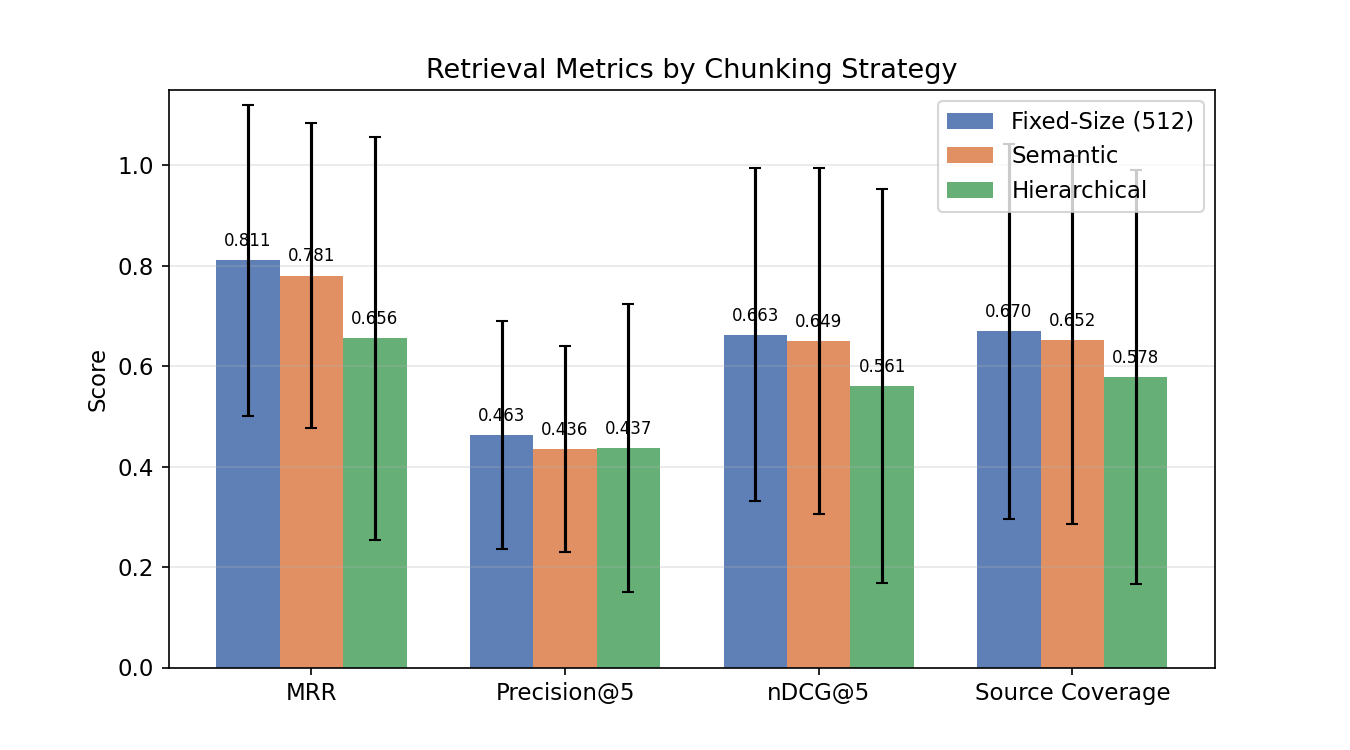
\includegraphics[width=\columnwidth]{figures/retrieval_metrics_comparison.png}}
\caption{Retrieval metrics comparison across the three chunking strategies. Fixed-size and semantic are close, while hierarchical lags behind.}
\label{fig:retrieval}
\end{figure}

% ============================================================
\section{Results and Discussion}

\subsection{What Worked Well}

\textbf{Hybrid retrieval} is effective. Combining dense and BM25 signals through RRF produces reliable results across all strategies. The $\alpha=0.7$ weighting favoring dense retrieval works well for our paraphrased queries.

\textbf{Fixed-size chunking} is a strong baseline. Despite its simplicity, it achieves the best overall MRR (0.811) and correctness (0.642). The 512-token chunk size provides enough context for the LLM while keeping chunks focused. This is consistent with findings in the chunking literature showing that fixed-size approaches often outperform more complex strategies on structured documents.

\textbf{Anti-hallucination guard} catches obvious citation errors. The programmatic citation verification strips invalid references and prevents the system from presenting answers with fabricated sources.

\textbf{Text mining features} provide useful corpus exploration. Keyword extraction reveals product-specific vocabulary, and the taxonomy classifier helps users understand which product categories contribute to a given answer.

\subsection{What Did Not Work}

\textbf{Hierarchical chunking underperforms.} Despite the theoretical appeal of separating retrieval precision (small children) from generation context (large parents), this strategy achieves the lowest MRR (0.656) and correctness (0.530). The likely reason is that IKEA buying guides have relatively flat document structure: they are short, single-topic PDFs without deep section hierarchies. The 128-token children are too small to contain discriminative terms for product-level queries, and the 1024-token parents sometimes span unrelated sections. This approach would likely work better on longer, more structured documents like academic papers or technical manuals.

\textbf{Semantic chunking has high size variance.} While semantic chunks have good boundary clarity (BC\,=\,0.931), the extreme size variance (3 to 3493 tokens) means some chunks are too large for effective retrieval and others are too small to carry meaningful content. A hybrid approach---semantic splitting followed by size constraints---would likely improve consistency.

\textbf{The LLM sometimes ignores retrieved context.} Two of our failure cases show the model claiming information is absent when it is clearly present in the context. This is a known limitation of smaller LLMs, especially with longer contexts or unfamiliar formatting (e.g., fraction characters like 4\textonehalf{}'').

\subsection{Limitations}

\begin{itemize}
    \item \textbf{Small LLM:} \texttt{llama-3.1-8b-instant} limits answer quality. A larger model (e.g., Llama 3.1 70B or GPT-4o) would likely improve correctness and reduce generation failures.
    \item \textbf{Citation F1 peaks at 0.52:} The model often cites the correct product but wrong guide (e.g., citing D20 instead of D02, both PAX-related).
    \item \textbf{LLM-as-judge bias:} We use the same model for generation and evaluation, which may introduce systematic bias. Human evaluation would provide more reliable quality assessments.
    \item \textbf{Corpus scope:} 20 buying guides covers the main product lines but not the full IKEA catalog. Scaling to hundreds of documents would test the system's retrieval robustness.
    \item \textbf{No re-ranking:} A cross-encoder re-ranker between retrieval and generation could improve precision, especially for comparative queries that need multiple relevant documents.
    \item \textbf{Citation extraction:} The regex used to extract document citations also matches dimension strings in product specifications (e.g., ``D38'' from depth measurements), which slightly inflates the incorrect citation count and deflates citation precision.
\end{itemize}

\begin{figure}[htbp]
\centerline{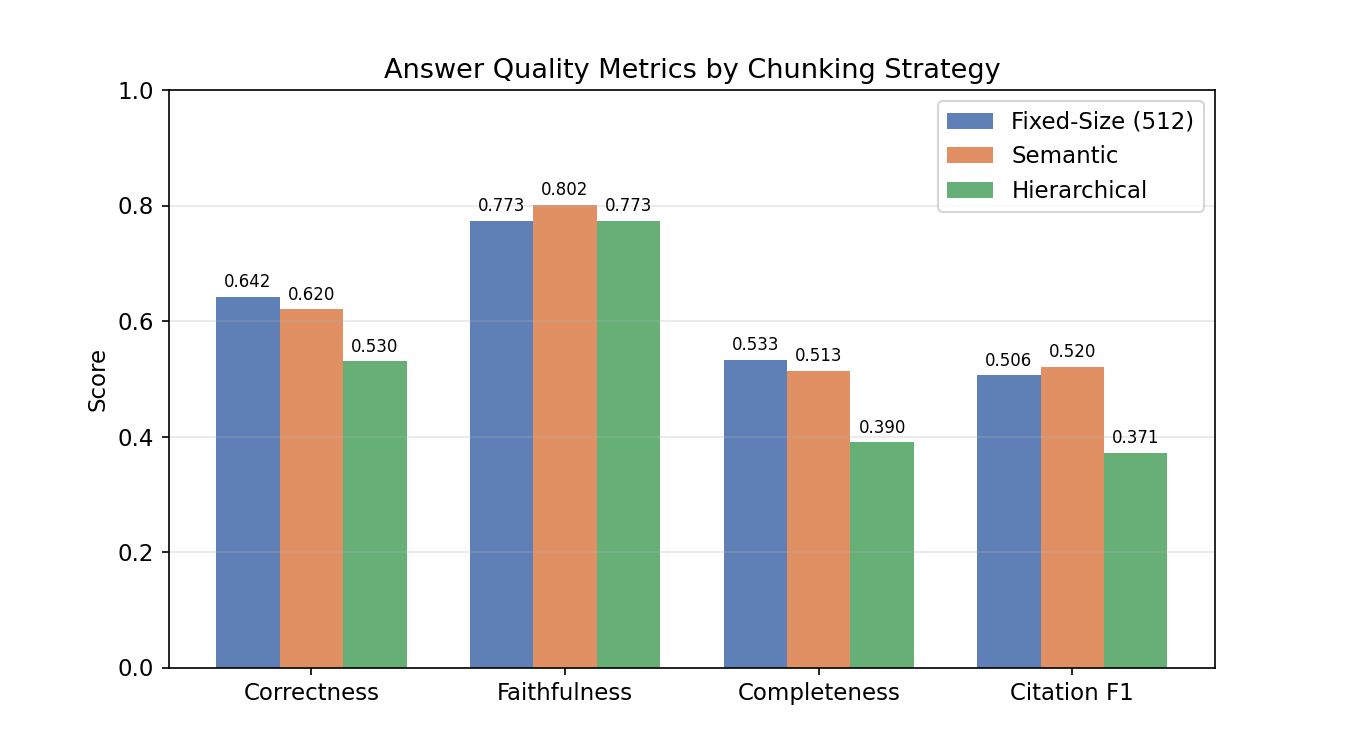
\includegraphics[width=\columnwidth]{figures/answer_quality_comparison.png}}
\caption{Answer quality metrics (correctness, faithfulness, completeness) across strategies. Semantic achieves the highest faithfulness.}
\label{fig:answer}
\end{figure}

% ============================================================
\section{Future Improvements}

Based on the observed limitations, we identify the following concrete improvements:

\textbf{Better retrieval.} Adding a cross-encoder re-ranker (e.g., \texttt{ms-marco-MiniLM-L-6-v2}) between retrieval and generation would re-score the top-$k$ candidates using full query-document interaction, improving precision for comparative queries that require multiple documents.

\textbf{Constrained semantic chunking.} Combining semantic breakpoints with minimum/maximum size constraints would preserve the boundary clarity advantage of semantic chunking while avoiding the extreme size variance that hurts retrieval consistency.

\textbf{Larger LLM.} Upgrading to a 70B+ parameter model would reduce the generation failures we observed, where the model ignores relevant context or hallucinates product details.

\textbf{Human evaluation.} Replacing or supplementing LLM-as-judge with human evaluation would provide more reliable quality assessments and eliminate the bias of using the same model for generation and evaluation.

\textbf{Query routing.} Different query types (factual vs.\ comparative vs.\ thematic) could benefit from different retrieval parameters (e.g., higher top-$k$ for comparative queries, lower for factual). A lightweight query classifier could route queries to appropriate retrieval configurations.

% ============================================================
\section{Conclusion}

We built FurnishRAG, a RAG system for answering questions about IKEA products using 20 buying guides. Our main contribution is a systematic comparison of three chunking strategies across 90 experiments.

The results show that \textbf{fixed-size chunking at 512 tokens is a strong default} for structured product documentation, achieving the best MRR (0.811) and correctness (0.642). Semantic chunking offers a slight advantage in faithfulness (0.802) but at the cost of high chunk size variance. Hierarchical parent-child chunking, despite its theoretical appeal, underperforms on short, flat documents like buying guides.

Our failure analysis reveals that both retrieval and generation contribute to failures: 4 of 7 failures are retrieval-side (MRR\,=\,0.0) and 3 involve generation limitations despite partial or full retrieval success. This suggests that improving retrieval---through re-ranking, query expansion, or adaptive top-$k$---and upgrading the LLM would both yield measurable gains.

The system demonstrates that RAG is effective for grounded question answering over product documentation, and that chunking strategy selection should consider document structure. Short, single-topic documents favor simpler chunking, while longer, hierarchically structured documents may benefit from parent-child approaches.

\begin{thebibliography}{00}
\bibitem{b1} P. Lewis, E. Perez, A. Piktus, F. Petroni, V. Karpukhin, N. Goyal, H. K\"{u}ttler, M. Lewis, W. Yih, T. Rockt\"{a}schel, S. Riedel, and D. Kiela, ``Retrieval-augmented generation for knowledge-intensive NLP tasks,'' in \textit{Proc. NeurIPS}, 2020.
\bibitem{b2} S. Robertson and H. Zaragoza, ``The probabilistic relevance framework: BM25 and beyond,'' \textit{Found. Trends Inf. Retr.}, vol. 3, no. 4, pp. 333--389, 2009.
\bibitem{b3} G. V. Cormack, C. L. A. Clarke, and S. B\"{u}ttcher, ``Reciprocal rank fusion outperforms condorcet and individual rank learning methods,'' in \textit{Proc. SIGIR}, 2009, pp. 758--759.
\bibitem{b4} N. Reimers and I. Gurevych, ``Sentence-BERT: sentence embeddings using Siamese BERT-networks,'' in \textit{Proc. EMNLP}, 2019.
\bibitem{b5} M. Grootendorst, ``BERTopic: neural topic modeling with a class-based TF-IDF procedure,'' 2022, arXiv:2203.05794.
\bibitem{b6} M. Grootendorst, ``KeyBERT: minimal keyword extraction with BERT,'' 2020. [Online]. Available: \url{https://github.com/MaartenGr/KeyBERT}
\bibitem{b7} S. Es, J. James, L. Espinosa-Anke, and S. Schockaert, ``RAGAS: automated evaluation of retrieval augmented generation,'' 2023, arXiv:2309.15217.
\bibitem{b8} Meta AI, ``Llama 3.1 model card,'' 2024. [Online]. Available: \url{https://github.com/meta-llama/llama-models}
\bibitem{b9} J. Chroma, ``ChromaDB: the AI-native open-source embedding database,'' 2024. [Online]. Available: \url{https://www.trychroma.com/}
\end{thebibliography}

\end{document}
